\begin{frame}
    \frametitle{Reactor Deployment}
    \begin{columns}
        \column[t]{5cm}
        \begin{itemize}
            \item The last \gls{LWR} is decommissied in 2076
            \item In the no growth scenarios (Scenarios 2, 3) the advanced reactors are 
                  deployed starting in July 2038
            \item In the 1\% growth scenarios (Scenarios 4, 5) the advanced reactors are 
                  deployed starting in Auggust 2036
            \item Scenario 2-5 require a maximum of 5962, 50, 11474, and 51 reactors
        \end{itemize}

        \column[t]{5cm}
        \begin{figure}
            \centering 
            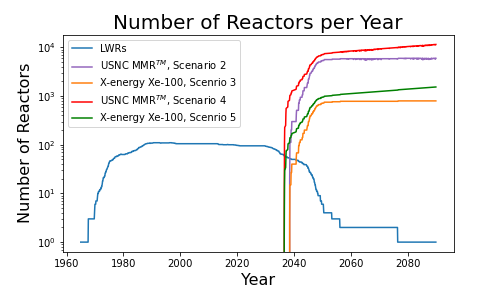
\includegraphics[scale=0.3]{figures/rxdeployment_scenarios_all.png}
            \caption{Energy produced per year by all reactors in each scenario.}
            \label{fig:rx_deployment}
        \end{figure}
    \end{columns}
\end{frame}

\begin{frame}
    \frametitle{Energy}
    \begin{columns}
        \column[t]{5cm}
        \begin{itemize}
            \item Small variations from demand in Scenarios 2 and 4 when 
                  reactors are deployed
        \end{itemize}

        \column[t]{5cm}
        \begin{figure}
            \centering 
            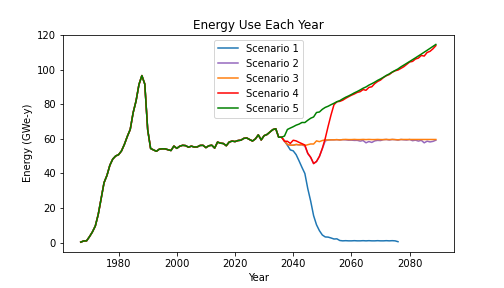
\includegraphics[scale=0.3]{figures/energy_scenarios_all.png}
            \caption{Energy produced per year by all reactors in each scenario.}
            \label{fig:energy}
        \end{figure}
    \end{columns}
\end{frame}

\begin{frame}
    \frametitle{Fresh Fuel Transactions}
    \begin{columns}
        \column[t]{5cm}

        \column[t]{5cm}
        \vspace{-0.8cm}
        \begin{figure}
            \centering 
            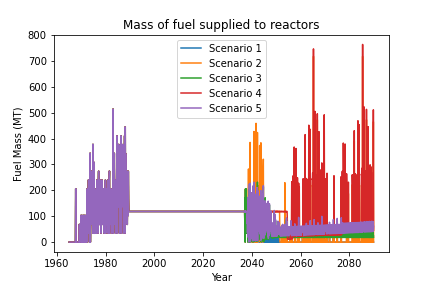
\includegraphics[scale=0.3]{figures/fuelsupply_scenarios_all.png}
            \caption{Energy produced per year by all reactors in each scenario.}
            \label{fig:fuel_allRX}
        \end{figure}
        \vspace{-0.8cm}
        \begin{figure}
            \centering 
            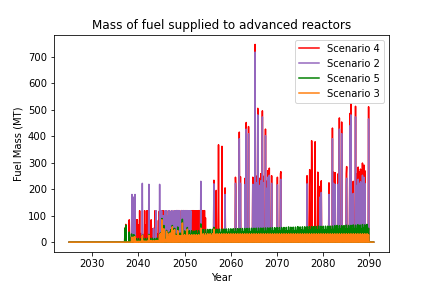
\includegraphics[scale=0.3]{figures/advancedRX_fuelsupply_scenarios_2-5.png}
            \vspace{0cm}
            \caption{Energy produced per year by all reactors in each scenario.}
            \label{fig:fuel_advancedRX}
        \end{figure}
    \end{columns}
    

\end{frame}

\begin{frame}
    \frametitle{\gls{SWU} Requirements}
    \begin{columns}
        \column[t]{5cm}

        \column[t]{5cm}
        \begin{figure}
            \centering 
            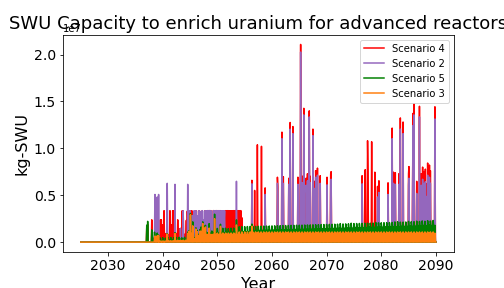
\includegraphics[scale=0.3]{figures/haleuSWU_scenarios_all.png}
            \caption{\gls{SWU} required to produce fuel for advanced reactors.}
            \label{fig:swu}
        \end{figure}
    \end{columns}
    

\end{frame}

